\chapter{Egobets}
\graphicspath{{/Users/brunomedina/Dropbox/Tesis-Egobets/egobets-notas/resources/diagramas/}}

Se describen las cuatro piezas de software desarrolladas que conforman en su totalidad el sistema de Egobets. Las tres primeras permiten al usuario adminstrativo echar a andar toda la maquinaria. Y la última pieza, conocida como el portal público, proporciona al usuario final los servicios del sistema a través de un sitio web usable, práctico y profesional. 
A todo este conjunto de herramientas y programas que el usuario necesita para esta tarea se le conocerá como \emph{Back Office}.

\section{Descripción General}
El ecosistema de Egobets consiste principalmente de cuatro piezas de software. Ver la figura~\ref{Fig:Sistemas}. 




\begin{figure}[!htb]\centering
   \begin {minipage}{1\textwidth}
     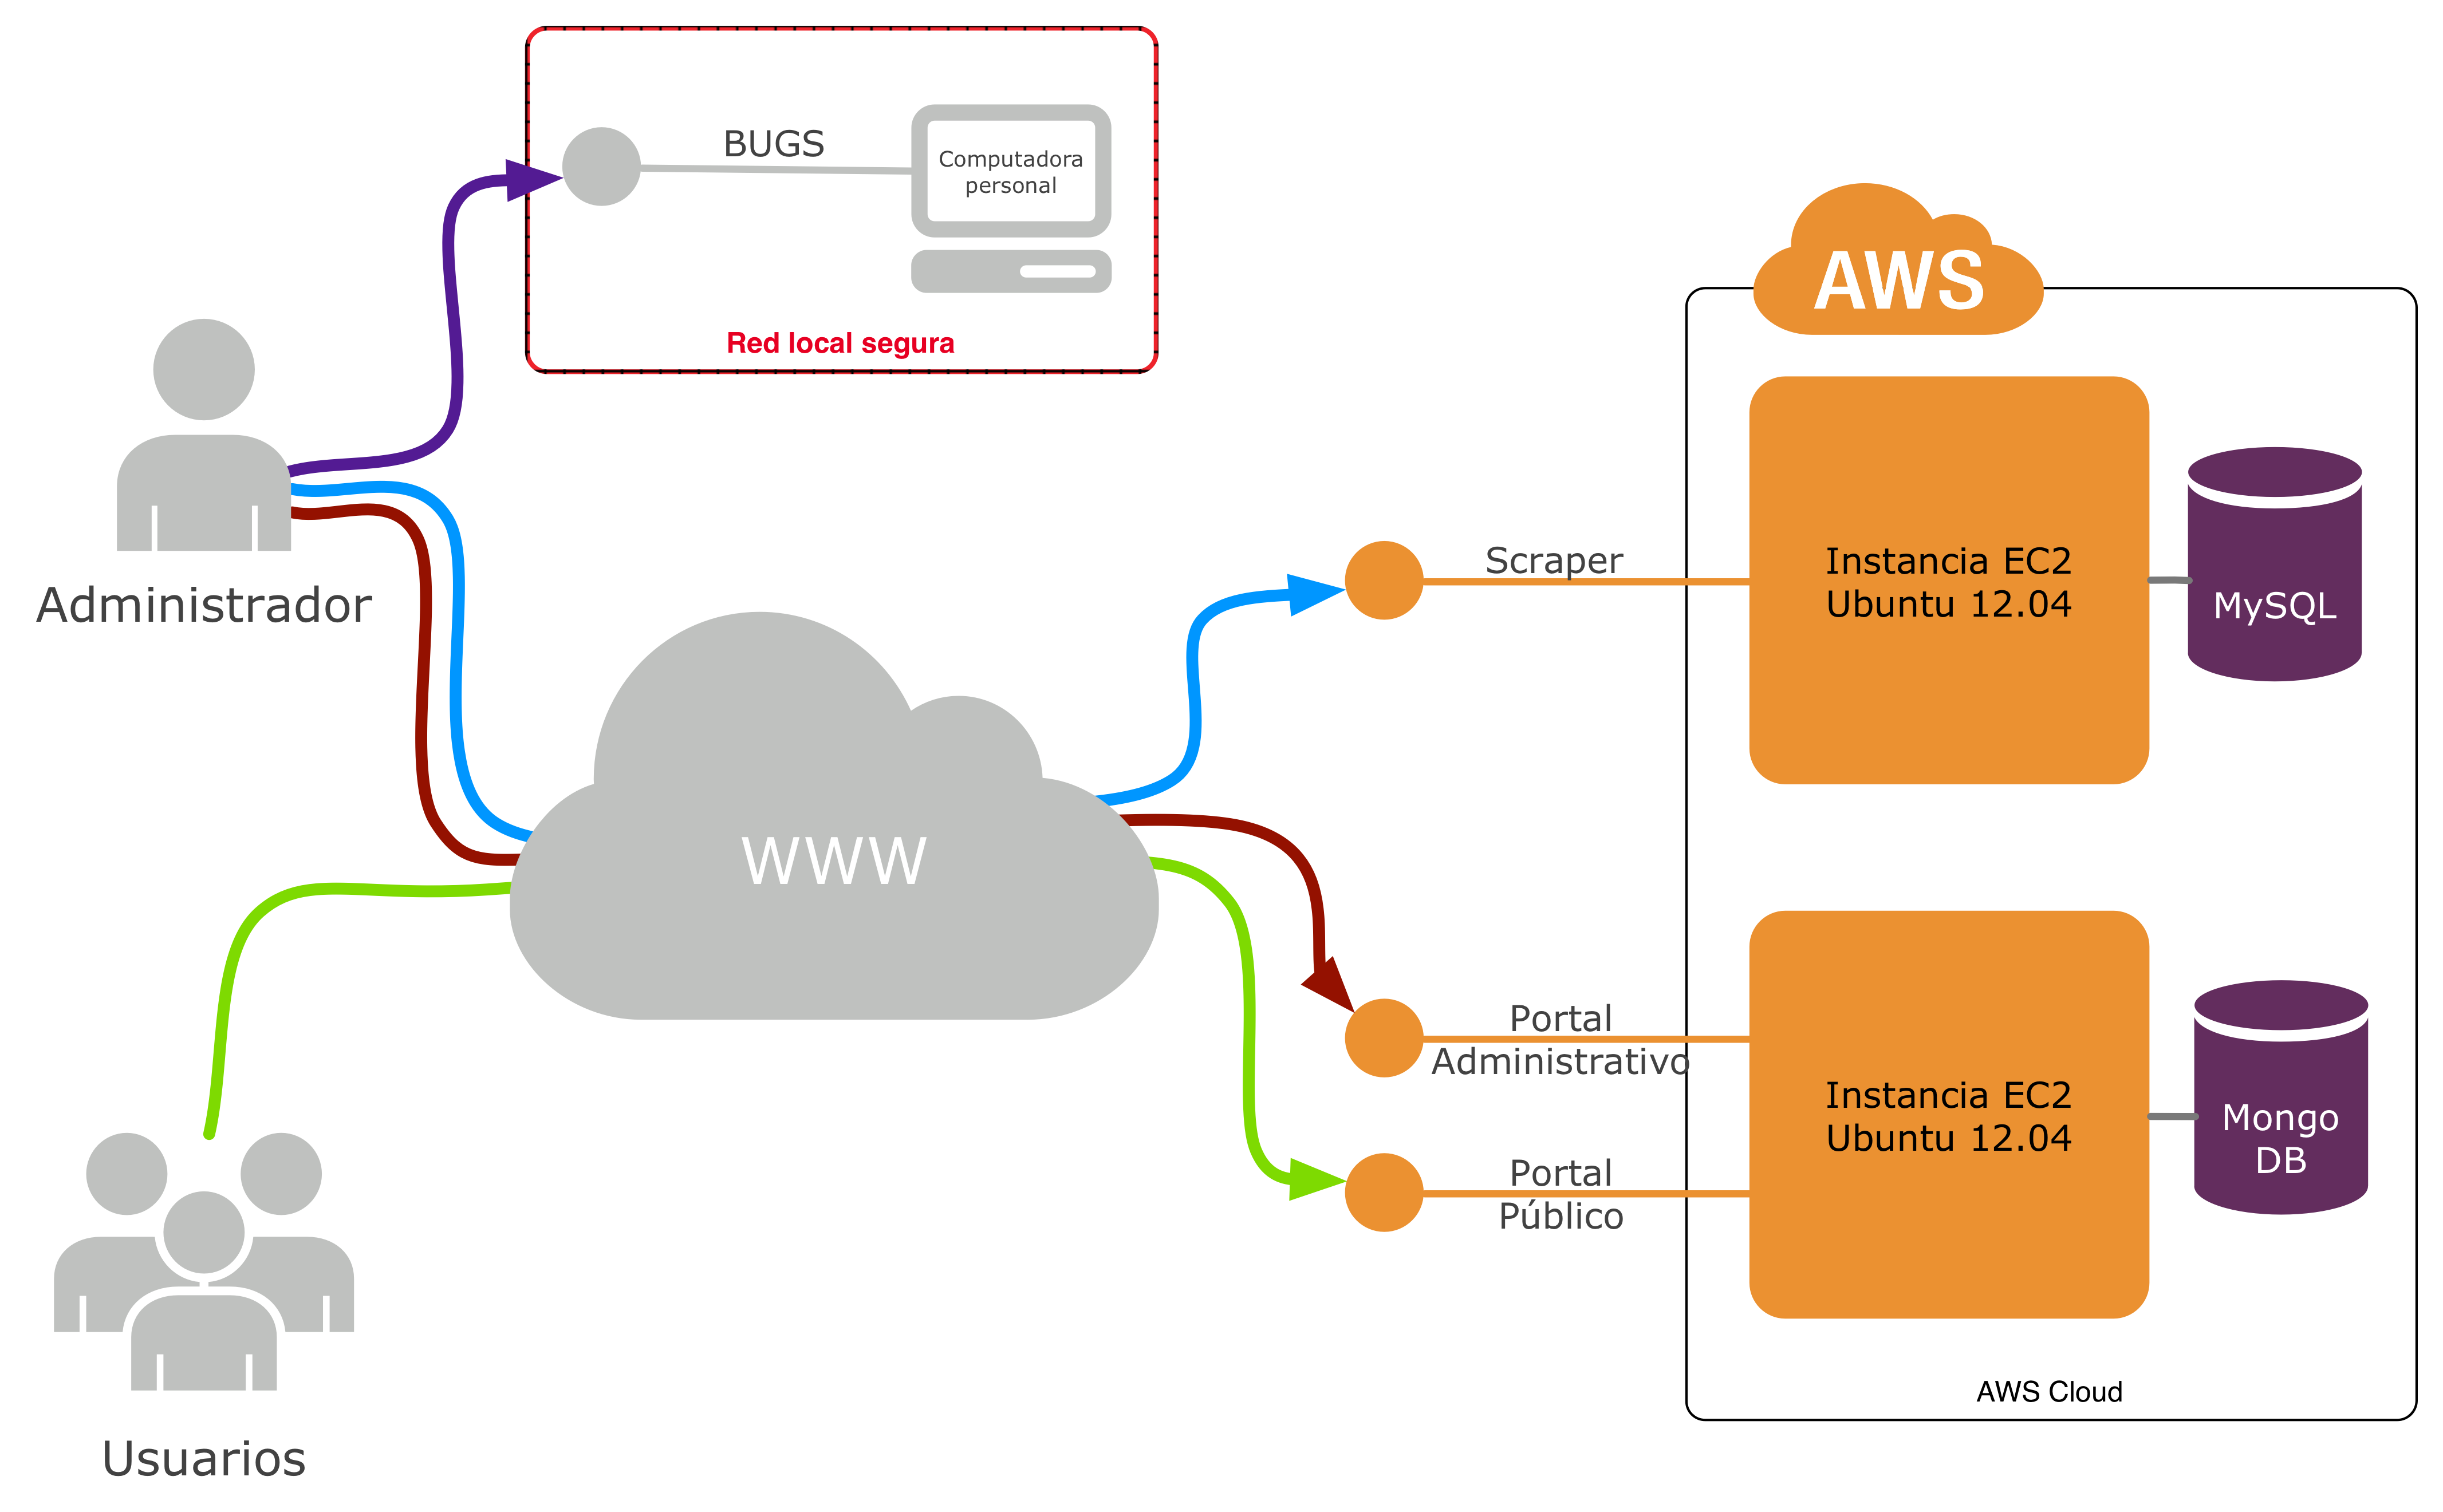
\includegraphics[width=\linewidth]{sistemas}
     \caption{Diagrama de sistemas y usuarios}\label{Fig:Sistemas}
   \end{minipage}
\end{figure}

El Sistema de recopilación de información y estadísiticas de los partidos (\emph{Sistema de recopilación}), el \emph{Portal administrativo} y el \emph{Portal público} corren bajo una arquitectura cliente servidor en la nube de Amazon Web Services; mientras que el Sistema de estimación de probabilidades (\emph{Sistema de estimación}) corre en un ordenador personal.


\subsubsection{Computación en la nube}

El sistema usa la nube para ofrecer sus servicio a los usuarios, se puede decir que el software corre en un esquema tipo ``SaaS''\footnote{Software as a Service. ``Es el más conocido de los niveles de cómputo en la nube. El SaaS es un modelo de distribución de software que proporciona a los clientes el acceso a éste a través de la red (generalmente Internet). De esta forma, ellos no tienen que preocuparse de la configuración, implementación o mantenimiento de las aplicaciones, ya que todas estas labores se vuelven responsabilidad del proveedor. Las aplicaciones distribuidas a través de un modelo de Software como Servicio pueden llegar a cualquier empresa sin importar su tamaño o ubicación geográfica.'' \cite{computoNube}.}, esto implica que el usuario simplemente ingresa a su cuenta en un navegador de internet y puede ver las asesorías para sus apuestas.
Del artículo ``Cómputo en Nube: Ventajas y Desventajas'' de Martínez y Gutiérrez \cite{computoNube}  se retoman las siguentes ventajas de este paradigma:
\begin{itemize}
	\item \textbf{Costos.} Podría ser la ventaja más atractiva que presenta el cómputo en la nube, y si no lo es, al menos es la más evidente de todas las que ofrece esta tecnología. Al dejar la responsabilidad de la implementación de la infraestructura al proveedor, el cliente no tiene que preocuparse por comprar equipos de cómputo, capacitar personal para la configuración y mantenimiento de éstos, y en algunos casos, por el desarrollo del software. Además el usuario de estos servicios únicamente paga por los recursos que utiliza, permitiéndole diseñar un plan de pago normalmente a partir del tiempo en que éste se utiliza (memoria, procesamiento, almacenamiento).

	\item \textbf{Competitividad.} Al no tener que adquirir equipos costosos, las pequeñas empresas pueden tener acceso a las más nuevas tecnologías a precios a su alcance pagando únicamente por consumo. De este modo las organizaciones de cualquier tipo podrían competir en igualdad de condiciones en áreas de TI con empresas de cualquier tamaño. La ventaja competitiva no está en aquel que tiene los recursos de cómputo sino en quien los emplea mejor.

	\item \textbf{Disponibilidad.} El proveedor está obligado a garantizar que el servicio siempre esté disponible para el cliente. En este sentido, la virtualización juega un papel fundamental, ya que el proveedor puede hacer uso de esta tecnología para diseñar una infraestructura redundante que le permita ofrecer un servicio constante de acuerdo a las especificaciones del cliente.


	\item \textbf{Abstracción de la parte técnica.} Como se mencionó al hablar de costos, el cómputo en la nube permite al cliente la posibilidad de olvidarse de la implementación, configuración y mantenimiento de equipos; transfiriendo esta responsabilidad al proveedor del servicio.

	\item \textbf{Acceso desde cualquier punto geográfico.} El uso de las aplicaciones diseñadas sobre el paradigma del cómputo en la nube puede ser accesible desde cualquier equipo de cómputo en el mundo que esté conectado a Internet. El acceso normalmente se hace desde un navegador web, lo que permite a la aplicación ser utilizada no únicamente desde una computadora de escritorio o una computadora portátil, sino que va más allá, permitiendo al usuario hacer uso de la aplicación incluso desde dispositivos móviles como smartphones.

	\item \textbf{Escalabilidad.} El cliente no tiene que preocuparse por actualizar el equipo de cómputo sobre el que se está corriendo la aplicación que utiliza, ni tampoco por la actualización de sistemas operativos o instalación de parches de seguridad, ya que es obligación del proveedor del servicio realizar este tipo de actualizaciones. Además, éstas son transparentes para el cliente, por lo que la aplicación debe de continuar disponible para el usuario en todo momento aún cuando se esté realizando el proceso de actualización del lado del proveedor. Las actualizaciones y nuevas funcionalidades son instaladas prácticamente de manera inmediata.

	\item \textbf{Disponibilidad.} El proveedor está obligado a garantizar que el servicio siempre esté disponible para el cliente. En este sentido, la virtualización juega un papel fundamental, ya que el proveedor puede hacer uso de esta tecnología para diseñar una infraestructura redundante que le permita ofrecer un servicio constante de acuerdo a las especificaciones del cliente.

\end{itemize}


\subsection{Proceso de generación de asesorías de apuestas}

\begin{figure}[!htb]\centering
   \begin {minipage}{1\textwidth}
     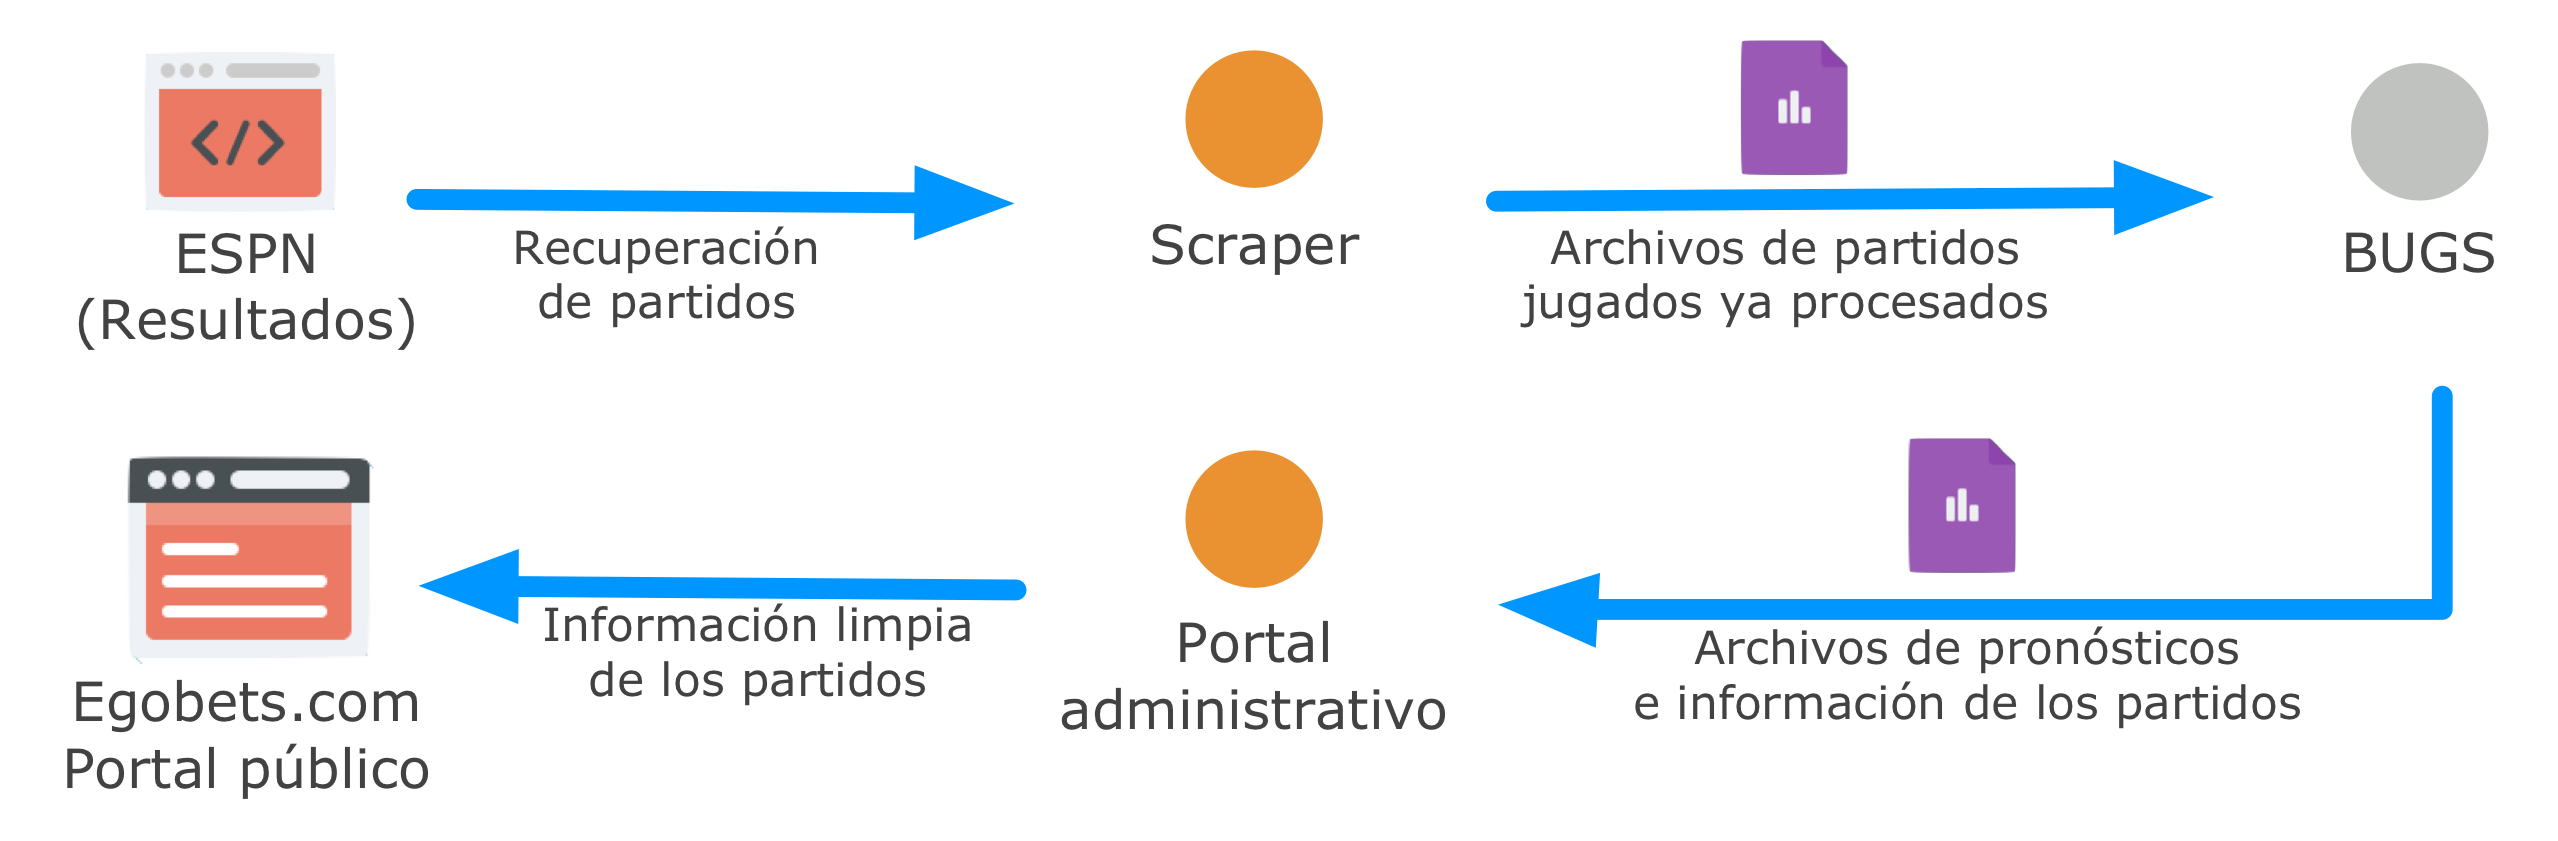
\includegraphics[width=\linewidth]{flujo}
     \caption{Diagrama de flujo de información}\label{Fig:flujo}
   \end{minipage}
\end{figure}

El proceso que se lleva a cabo en el \emph{Back Office} para alimentar el \emph{Portal público} (Ver la figura~\ref{Fig:flujo}), se puede describir de la siguiente manera:
\begin{enumerate}
	\item A través del \emph{Sistema de recopilación} los administradores descargan de la página de Internet de ESPN los resultados de todos los partidos de la temporada junto con la información de los próximos partidos por jugar  de cada una de las ligas Europeas.
	\item Los datos recopilados permiten a los administradores generar un conjunto de archivos de texto con toda la información de los resultados de los últimos partidos y las fechas de los próximos partidos.
	\item Los administradores usan estos archivos para alimentar el \emph{Sistema de estimación} y calcular los pronósticos de los próximos partidos y las probabilidades de los resultados.
	\item Se obtienen los archivos que contienen la información de los próximos partidos así como la información de los equipos por liga y su desempeño en la temporada en curso.
	\item En el \emph{Portal administrativo} se ingestan los archivos obtenidos con la información de los próximos partidos, resultados de partidos anteriores y las estadísticas de los equipos en la temporada en curso.
	\item Finalmente, con la nueva información ingresada, los usuarios podrán disfrutar en el \emph{Portal público} sus recomendaciones peronalizadas de apuestas.
\end{enumerate}


\subsection{Sistema de recopilación de información y estadísticas de los partidos}
\graphicspath{{/Users/brunomedina/Dropbox/Tesis-Egobets/egobets-notas/resources/recopilador/}}
Se desarrolló un sistema web que recupera al principio de cada temporada todos los partidos que se hayan jugado la temporada pasada y las fechas de los próximos partidos por jugar de cada una de las ligas. Para lograr la extracción de esta información el sistema cuenta con un ``Web Scraper'' que consigue la información de la página de ESPN y la transforma en objetos que después pueden ser ingestados en la base de datos. Finalmente, esta información se organiza en un documento CSV para ser descargado por los administradores.

\subsubsection{Tecnologías destacadas}

\begin{itemize}
	\item \textbf{Servidor LAMP.} Esta es una de las configuraciones más populares para servidores web. El famoso acrónimo representa lo siguiente:
	\begin{itemize}
		\item Linux. Sistema operativo Linux, en específico se utiliza la versión de Ubuntu LTS 12.04. Esta versión es estable con una gran comunidad activa de soporte.
		\item Apache. El servidor HTTP, encargado de recibir y procesar las llamadas http.
		\item MySQL. Base de datos relacional que permite al sistema persistir toda la información recuperada del internet.
		\item PHP. El lenguaje de programación web más utilizado en el mercado \cite{(REFERENCIA)}. PHP es conocido por ....
		sus principales ventajas son los bajos costos de mantenimiento, ....
	\end{itemize}
	
	\item Code Igniter. Es un framework\footnote{conjunto de herramientas de trabajo. All of them offer you chunks of pre-written code that make the repetitive or complex processes of coding easier, and impose a helpful structure on your site development.
} de PHP que ahorra tiempo en le programación, robustece tu sistema y permite al programador alcanzar un grado mayor de sofisticación en su código. Uno de los puntos interesantes de este framework es que utiliza el patrón de diseño conocido como Modelo Vista Controlador (MVC), este patrón fue descrito por el noruego Trygve Reenskaug en 1979. 
	\begin{itemize}
		\item Modelos, son objetos que representan los datos. Estos objetos reflejan las tabla de la base de datos y pueden modificarla conforme sea requerido. Los modelos también realizan operacioens a los datos según sea necesario.
		\item Vistas, reflejan el estado del modelo. Son las responsables de desplegar la información al usuario final. En este caso específico, todas las vistas son representaciones HTML del contenido.
		\item Controladore, ofrecen opciones para cambiar el estado del modelo. Son los encargados de consultar los modelos. Proveen a las vistas los datos dinámicos a mostrar.
	\end{itemize}
	\cite{upton2007codeigniter}
	\item PHP Simple HTML DOM Parser
	\cite{chen2009php} \cite{chowdhury2014intelwiki}
	\item Bootstrap \cite{otto2010bootstrap}
	\cite{cochran2012twitter}
	
\end{itemize}

\subsubsection{Web Scraper}
Es un script que 
\cite{hogue2005thresher}
Definir lo que es un scraper

Definir las páginas que se buscan y como se recorren

Definir los objetos finales de la base de datos que se consumen.




\subsubsection{Descripción de su funcionamiento}

\begin{enumerate}
	\item \textbf{Equipos de la temporada.}
	Para poder comenzar la recuperación de información, es importante contar con los equipos que estén jugando esta temporada. Dependiendo de los resultados de la temporada anterior, los equipos que hayan quedado hasta abajo en la tabla de posición descienden a ligas menores y a su vez suben los mejores de estas ligas. Ver figura~\ref{Fig:los-equipos}
	\begin{figure}[!htb]\centering
	   \begin {minipage}{1\textwidth}
	     \frame{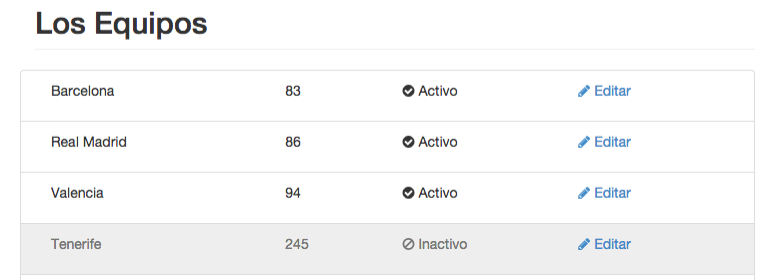
\includegraphics[width=\linewidth]{los-equipos}}
	     \caption[Ejemplo de equipos de la liga española]{Ejemplo de equipos de la liga española\footnotemark }\label{Fig:los-equipos}
	   \end{minipage}
	\end{figure}

	
	\item \textbf{Calendario de próximos partidos.}
	\begin{figure}[!htb]\centering
	   \begin {minipage}{1\textwidth}
	     \frame{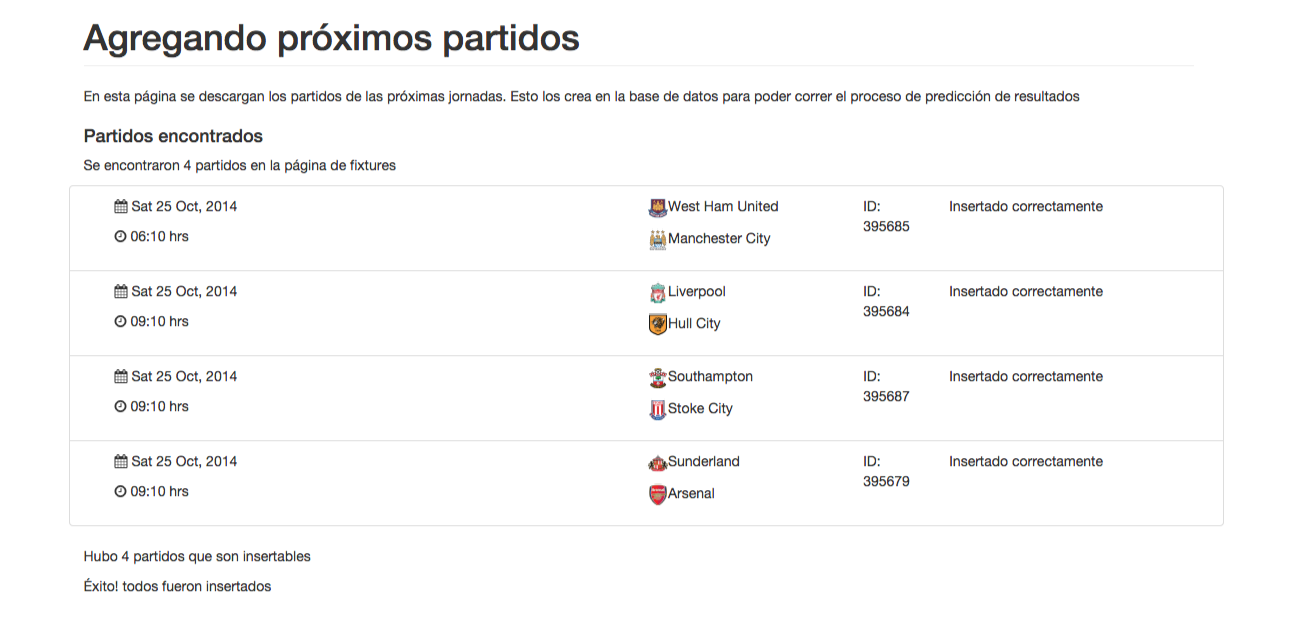
\includegraphics[width=\linewidth]{proximos-partidos}}
	     \caption{Recuperación de próximos partidos}\label{Fig:proximos-partidos}
	   \end{minipage}
	\end{figure}
	
	\item \textbf{Estadísticas e información de partidos jugados.}
	\begin{figure}[!htb]\centering
	   \begin {minipage}{1\textwidth}
	     \frame{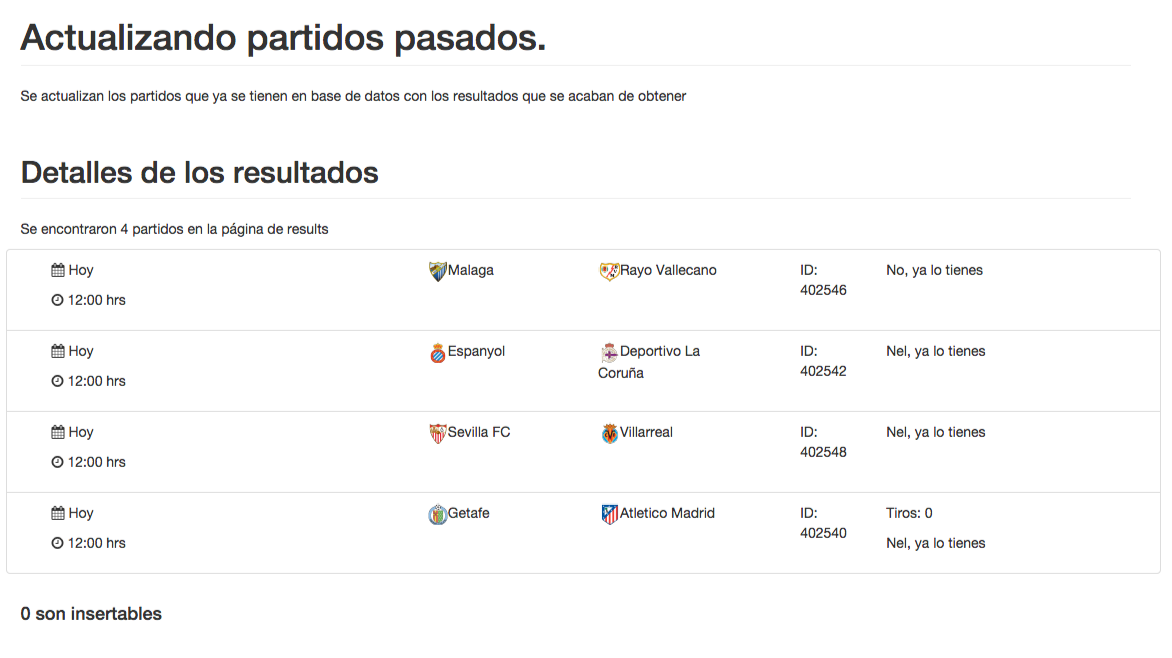
\includegraphics[width=\linewidth]{pasados-partidos}}
	     \caption{Recuperación de resultados de partidos ya jugados}\label{Fig:pasados-partidos}
	   \end{minipage}
	\end{figure}
	\item \textbf{Generación de archivos con resultados.}
	Es importante mencionar que se usan aproximadamente los últimos quinientos partidos para la generación de los archivos, esto implica que se deben tener en base de datos los equipos que participaron en las pasadas dos temporadas de juegos. Por este motivo de pueden encontrar equipos que se encuentran en el sistema con la bandera de inactivos.
	
\end{enumerate}













\subsection{Sistema de estimación de probabilidades}
Adicionalmente en esta sección se describirá el funcionamiento del Sistema de Estimación. Sin embargo, al ser un conjunto de programas en \emph{Fortran} que son ajenos al autor, no se profundizará en los detalles del desarrollo del mismo. Sin embargo, se dará la pauta para entender como se podrían generar probabilidades y pronósticos de los partidos.

\subsubsection{Predicciones}



\cite{rue2000prediction}

\cite{baio2010bayesian}

\cite{dixon2004value}

\cite{koopman2013dynamic}

 \subsubsection{Tecnologías destacadas}

\begin{itemize}
	\item \textbf{Fortran}
	\cite{robison1996c++}
	\cite{veldhuizen1997will}
\end{itemize}
	
\subsubsection{Descripción de su funcionamiento}

Montecarlo
Poisson
Nonormal
Markov


\subsection{Portal administrativo}

\subsubsection{Sitio web para los administradores}

 \cite{alfredo2005ingenieria}
 
 \subsubsection{Tecnologías destacadas}
 
 \begin{itemize}
 	\item LNNP
 	\item Code Igniter
 	\item Raphael
 \end{itemize}
 
 \subsubsection{Diagrama de base de datos}
 
 \subsubsection{Descripciónde su funcionamiento}
 
 \begin{itemize}
 	\item CRUD
 	\item Ingesta de archivos
	
 \end{itemize}
 

\section{Portal público Egobets.com}

\subsection{Características principales}
\subsubsection{Sitio web para los jugadores}
\subsubsection{Tecnologías destacadas}
 
 \begin{itemize}
 	\item LNNP
 	\item Code Igniter
 	\item Parallax
 \end{itemize}
  
\subsubsection{Módulos}

 \begin{itemize}
 	\item Tablero
 	\item Mis Equipos
 	\item Ligas
 	\item Partidos
 	\item Perfil
 	\item Pagos
 	\item Perfil de riesgo
 	\item Sistemas de reserva
 \end{itemize}
 
\subsection{Encuestas de adversidad al riesgo}
\subsection{Ahorro precaucional}

Supongamos $F_1,...,F_n$ distribuciones y la siguiente sucesión de Variables aleatorias $(x_1^t)_{t=1}^{\infty},..., (x_n^t)_{t=n}^{\infty}$ independientes $x_j^{t} \sim F_j \,\forall\, t\, \in\, \mathbb{N}$.\\

Sean $\alpha_1,..., \alpha_n\,\in\,\Re^+\,\, \cdot \ni \cdot \,\,\displaystyle \sum_{j=1}^n\alpha_j=1$, definimos:

\begin{itemize}
 \item $z_1=\displaystyle \sum_{j=1}^n\alpha_jx_j'$ 
 \item $z_{t+1}=\displaystyle \sum_{j=1}^n\alpha_jx_j^{t+1}+z_t$ 
\end{itemize}
Supongamos que $E[x_j^t]>1\,\,\forall\,t \,\in\,\mathbb{N}\rightarrow E[z_t]=tE[z_1]=t\mu>1$\\

{\bf Problema:}\\
Encontrar $y \,\,\cdot \ni\cdot\,\,(1-ty)+yz_t \ge y\,\,\forall\,t\,\in \mathbb{N}$ con probabilidad $(1-\alpha)\times 100\%$. $(y\in[0,1])$.

$$\rightarrow y z_t\ge (t+1)y-1\quad\rightarrow\quad z_t\ge(t+1)-\frac{1}{y}$$
$$\qquad\qquad\qquad\qquad\qquad\qquad\qquad\,\,\rightarrow z_t\ge t+k (con\,\,\,k=1-\frac{1}{y})$$

equivalentemente: Encontrar $k\le 0\,\,\cdot\ni\cdot\,\,z_t\ge t+k\,\,\forall\,t\in\mathbb{N}$ con probabilidad $(1-\alpha)\times 100\%$.\\

Sol: \\
Sea $\mu=E[z_1]$, $\sigma^2=Var[z_1]$\\

\[\rightarrow (1-\alpha)=p(z_t)\ge t+k\,\,\forall\,\in\mathbb{N}\qquad\qquad\qquad\qquad\qquad\qquad\qquad\qquad\quad\quad\]
\[=p(z_1\ge 1+k)\cdot p(z_2\ge 2+k\,\,|z_1\ge 1+k)\cdots\qquad\quad\]
\[=p(z_1\ge 1+k)\cdot\displaystyle\prod_{t=1}^{\infty}p(z_{t+1}\ge (t+1)+k\,|z_t\ge t+k)\]\\

Usando el T.C.L.: $z_t \rightarrow N(t\mu,\,t\sigma^2)\,\,\forall\,t\in\,\mathbb{N}$

\begin{enumerate}[(i)]
 \item $p(z_1\ge 1+k)=p{\displaystyle\left(\frac{z_1-\mu}{\sigma}\ge\frac{(1+k)-\mu}{\sigma}\right)=1-\Phi\left(\frac{k-(\mu-1)}{\sqrt{t}\sigma}\right)}$\\
 
 \item $p(z_{t+1}\ge (t+1)+k\,|z_t\ge t+k)=\displaystyle\frac{p(z_{t+1}\ge (t+1)+k,\,z_t\ge t+k)}{p(z_t\ge t+k)}$\\
 
    \begin{itemize}
     \item $p(z_t\ge t+k)=p{\displaystyle\left(\frac{z_t-t\mu}{\sqrt{t}\sigma}\ge\frac{k-t(\mu-1)}{\sqrt{t}\sigma}\right)}$\\
     
     $\qquad\qquad\qquad={\displaystyle 1-\Phi\left(\frac{k-t(\mu-1)}{\sqrt{t}\sigma}\right)}$\\
     
     \item $z_{t+1}=y_t+z_t$ con $y_t \sim (\mu,\sigma^2),\,\,y_t,z_t$ independientes\\ $z_t\sim(t\mu,t\sigma^2)$
    \end{itemize}
$\rightarrow f(y_t,z_t)\simeq \displaystyle\frac{1}{2\pi\sqrt{t}\sigma^2}\exp\{-\frac{1}{2\sigma^2}[(y_t-\mu)^2+\frac{1}{t}(z_t-t\mu)^2]\}$
\end{enumerate}

Sea \[\omega_t=y_t+z_t\qquad\qquad y_t=\omega_t-v_t\]
%\[\rightarrow\]
\[v_t=z_t\qquad\qquad z_t=v_t\]

\[\rightarrow J=\left( {1\atop 0} {-1\atop {1}} \right)\rightarrow |det(J)|=1\]

\[f(z_{t+1}z_t)=\displaystyle\frac{1}{2\pi\sqrt{t}\sigma^2}\exp\{\displaystyle -\frac{1}{2\sigma^2}[(z_{t+1}-z_t-\mu)^2+\frac{1}{t}(z_t-t\mu)^2]\}\]\\

$\rightarrow p(z_{t+1})\ge (t+1)+k,\,z_t\ge t+k$\\

\[={\displaystyle\int_{t+k}^{\infty}\int_{t+1+k}^{\infty}\frac{1}{2\pi\sqrt{t}\sigma^2}\exp\{\displaystyle -\frac{1}{2\sigma^2}[(z_{t+1}-z_t-\mu)^2+\frac{1}{t}(z_t-t\mu)^2]\}}dz_{t+1}dz_t\]\\

\[{=\displaystyle\frac{1}{2\pi\sqrt{t}\sigma^2}\int_{t+k}^{\infty}\exp\{-\frac{1}{2\sigma^2 t}(z_t-t\mu)^2\}\int_{t+1+k}^{\infty}\frac{1}{\sqrt{2\pi}\sigma}\exp\{\displaystyle -\frac{1}{2\sigma^2}[(z_{t+1}-z_t-\mu)^2\}dz_{t+1}dz_t}\]\\

\newpage

\[\footnote{Ver Apéndice A}= {\displaystyle\frac{1}{2\pi\sqrt{t}\sigma^2}\int_{t+k}^{\infty}\exp\{-\frac{1}{2\sigma^2 t}(z_t-t\mu)^2\}\left[1-\Phi\left(\frac{k+t-z_t-(\mu-1)}{\sigma}\right)\right]}\]

 \rule{14cm}{0.1mm}
\[\overline{z_t}=\frac{1}{t}z_t,\,\,\,d\overline{z_t}=\frac{1}{t}dz_t,\,\,\,(\overline{z_t})_0=1+\frac{k}{t},\,\,\,(\overline{z_t})_1=\infty\]
 \rule{14cm}{0.1mm}

\[={\displaystyle\frac{\sqrt{t}}{2\pi\sqrt{t}\sigma^2}\int_{1+k/t}^{\infty}\exp\{-\frac{t}{2\sigma^2 }(\overline{z}_t-\mu)^2\}\left[1-\Phi\left(\frac{k+t(1-\overline{z}_t)-(\mu-1)}{\sigma}\right)\right]d\overline{z}_t}\]

Por tanto:\\

$p(z_{t+1})\ge (t+1)+k,\,z_t\ge t+k$\\

\[\simeq {\displaystyle \frac{\sqrt{t}\int_{1+k/t}^{\infty}\exp\{-\frac{t}{2\sigma^2 }(\overline{z}_t-\mu)^2\}\left[1-\Phi\left(\frac{k+t(1-\overline{z}_t)-(\mu-1)}{\sigma}\right)\right]d\overline{z}_t}{\sqrt{2\pi}\sigma\left(1-\Phi\left(\frac{k-t(\mu-1)}{\sqrt{t}\sigma}\right)\right)}}\]

Para calcular $k$ se resuelve la siguiente ecuación:

\[\log (1-\alpha)=\log(p|z_1\ge 1+k)+\displaystyle\sum_{t=1}^{\infty}\log(p(z_{t+1})\ge (t+1)+k,\,z_t\ge t+k)\]

\[y=\frac{1}{1-k}\]

Se realizó una muestra $y_1,..., y_n$, donde:

\[y_1=CA(p_i,\mu_i,\sigma_i)\]

Donde:
\begin{itemize}
 \item $p_i$: Un valor de probabilidad deseado.
 \item $M_i$: Un valor de $E[z_1]$ dado.
 \item $\delta_i$: Un valorde $Var(z_i)^{1/2}$.
 \item $CA$: La función que se define implícitamente de resolver las ecuaciones para calcular la cantidad de apostar.
\end{itemize}

A tales datos se les ajustó el siguiente modelo lineal:

\[y_i=\beta_0+\beta_1p_i+\beta_2\mu_i+\beta_3\sigma_i+\varepsilon_i\]

\newpage

El ajuste es el siguiente:

\begin{itemize}
 \item $\beta_0=0.2925$
  \item $\beta_1=-0.9975$
 \item $\beta_2=1.3772$
 \item $\beta_3=-1.1127$
\end{itemize}

Con $R^2=0.95$.\\

En adelante, se tomará como aproximación lo siguiente:

\[CA(p,\mu,\sigma)\simeq0.2925-0.9975p+1.3772\mu-1.1127\sigma\]

\subsection{Asesoría de apuestas}
{\bf Problema:} Decidir $p$ de manera óptima.\\

Sea $x$ la cantidad de ingresos restantes ($o\ge x\ge1$, en porcentaje), y $\mu$, $\sigma$ la media y la desviación estandar de apostar en un periodo dados.\\

Supongamos $U_1,U_2: \Re^+\rightarrow \Re^+$ funciones de utilidad del dinero. ($U_1$ ganancias, $-U_2$ pérdidas) $\cdot\ni\cdot$ son no decrecientes y una vez continuamente diferenciables. Considerese la siguiente función:\\

\[f(p;x,\mu,\sigma)=[beneficio]-[costo]\]
\[f(p;x,\mu,\sigma)=[pU_1(y(p,\mu,\sigma)\mu x)]-[(1-p)U_2(x)]\]\\

Suponiendo $y(p,\mu,\sigma)=a_0-a_1p+a_2\mu-a_3\sigma$ se obtiene:\\

$a_i\ge 0,\,\,i=0,...,3$
\[f=pU_1((a_0-a_1p+a_2\mu-a_3\sigma)\mu x)-(1-p)U_2(x)\]

El problema es:\\

$max\,\,f$\\

Sol:\\

\[f'(p)=-pU_1'((a_0-a_1p+a_2\mu-a_3\sigma)\mu x)a_1\mu x\]
\[\qquad\qquad\qquad+U_1((a_0-a_1p+a_2\mu-a_3\sigma)\mu x)+U_2(x)=0\]

Si $U_1$ es cóncava $\rightarrow$ $p^*$ es un maximizador.\\

 Forma aproximada de obtener $p$ :
 
 \[y=a_0-a_1p+a_2\mu-a_3\sigma\]
 
 $\rightarrow$ Sea $b=a_1\mu x$, $p_0$ una aproximación de $p$. Definimos:
 
 \[\omega=y\mu x,\quad \omega_0=y(p_0,\mu,\sigma)\mu x\]
 
 \[\rightarrow U_1(\omega)=U_1(\omega_0)+U'_1(\omega_0)(\omega-\omega_0)+O((\omega-\omega_0))\] 
 \[=U_1(\omega_0)+bU'_1(\omega_0)(\omega_0)(p-p_0)+O((\omega-\omega_0))\]
 
 Se puede aproximar $f$ por:
 
 \[f(p)\simeq p[U_1(\omega_0)+bU'_1(\omega_0)(\omega_0)(p-p_0)]-(1-p)U_2(x)\]
 
 \[\Rightarrow f'(p)\simeq U_1(\omega_0)-2bU'_1(\omega_0)p+bU'_1(\omega_0)p_0+U_2(x)=0\]
 
 \[\Rightarrow p\simeq \frac{1}{2bU'_1(\omega_0)}[U_1(\omega_0)+U_2(x)]+\frac{1}{2}p_0\]
 
Supongamos $U_1:\Re^+ \rightarrow \Re^+$ dada por $U(\omega)=\omega^\alpha\qquad(0<\alpha\le1)$ y $U_2(x)=\beta x$\\

Notese que:
\begin{itemize}
 \item ${\displaystyle\frac{U_1(\omega_0)}{U'_1(\omega_0)}=\frac{\omega_0}{\alpha}}$
 \item ${\displaystyle\frac{\omega_0}{b}=\frac{a_0-a_1p+a_2\mu-a_3\sigma}{a_1}}$
\end{itemize}

\[\Rightarrow p\simeq \frac{1}{2\alpha a_1}[a_0+a_2\mu-a_3\sigma+\frac{\beta}{\mu}[(a_0-a_1p_0+a_2\mu-a_3\sigma)\mu x]^{1-\alpha}]+\frac{1}{2}(1-\frac{1}{\alpha})p_0\]
 
Supongamos ahora que $f$ es de la siguiente forma:

\[f(p)=pU_1(y(p,\mu,\sigma)\cdot \mu x)-(1-p)U_2(x)-pU_3(\theta(k\sigma-\mu))\]
 
i.e. Hay pérdidas potenciales por el riesgo de la inversión considerar
\[U_3(\theta(k\sigma-\mu))U_2(\theta(k\sigma-\mu)x)I(\theta(k\sigma-\mu)\ge 0)\]
 
$\Rightarrow$ De manera análoga se obtiene:

\[p\simeq\frac{1}{2bU'(\omega_0)}[U_1(\omega_0)+U_2(x)+U_2(\theta(k\sigma-\mu)xI_{\{m\ge0\}}]+\frac{1}{2}p_0\]
 
\newpage 
Si tomamos $U_1(\omega)0\omega^\alpha$, $U_2(x)=\beta x$ \\\\
 
$p\simeq \frac{1}{2\alpha a_1}\{(a_0+a_2\mu-a_3\sigma)$
\[+\frac{\beta_1}{\mu}[1+(\beta_2\sigma-\beta_3 \mu)I_{\{m\ge0\}}][(a_0-a_1p+a_2\mu-a_3\sigma)\mu x]^{1-\alpha}\}+\frac{1}{2}(1-\frac{1}{\alpha})p_0\] 


